\documentclass[24pt, a2papper, portrait]{tikzposter}
\usepackage[utf8]{inputenc}

\title{Computing forever}
\author{Alexander Aksentyev}
\date{\today}
\institute{National Research Nuclear University ``MEPhI''}

\usepackage{graphicx}
\usepackage{comment}
\usepackage{url}
\usepackage{tikz}
\usetikzlibrary{mindmap, trees, positioning, fit}
\usepackage{makecell}

\usetheme{Simple}

\tikzstyle{num} = [circle,text width=]
\tikzstyle{img} = [text width=]
\tikzstyle{note} = [fill=yellow!30, rectangle, rounded corners, text width=]

\begin{document}
	\maketitle
	\begin{columns}
		\column{.5}
			\block{Artificial Neural Networks}{
			\begin{tikzpicture}
			\begin{scope}[num/.append style={fill=green!20}]
			\node [img] (BN) {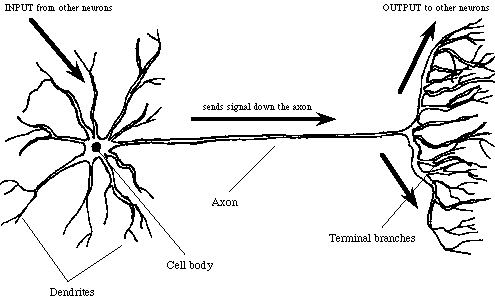
\includegraphics[scale=2]{BrainNeuron}};
			\node[num, anchor=west] at(BN.north east) {\makecell[c]{\textbf{100 billion}\\ neurons\\ in the brain}};
			\node [num, anchor=west] at(BN.south east) (con) {\makecell[c]{each one\\ connected to\\ \textbf{10,000}\\ neighbors}};
			\end{scope}
			\begin{scope}[num/.append style={fill=blue!20}]
			\node [img, below=7of BN] (ANN) {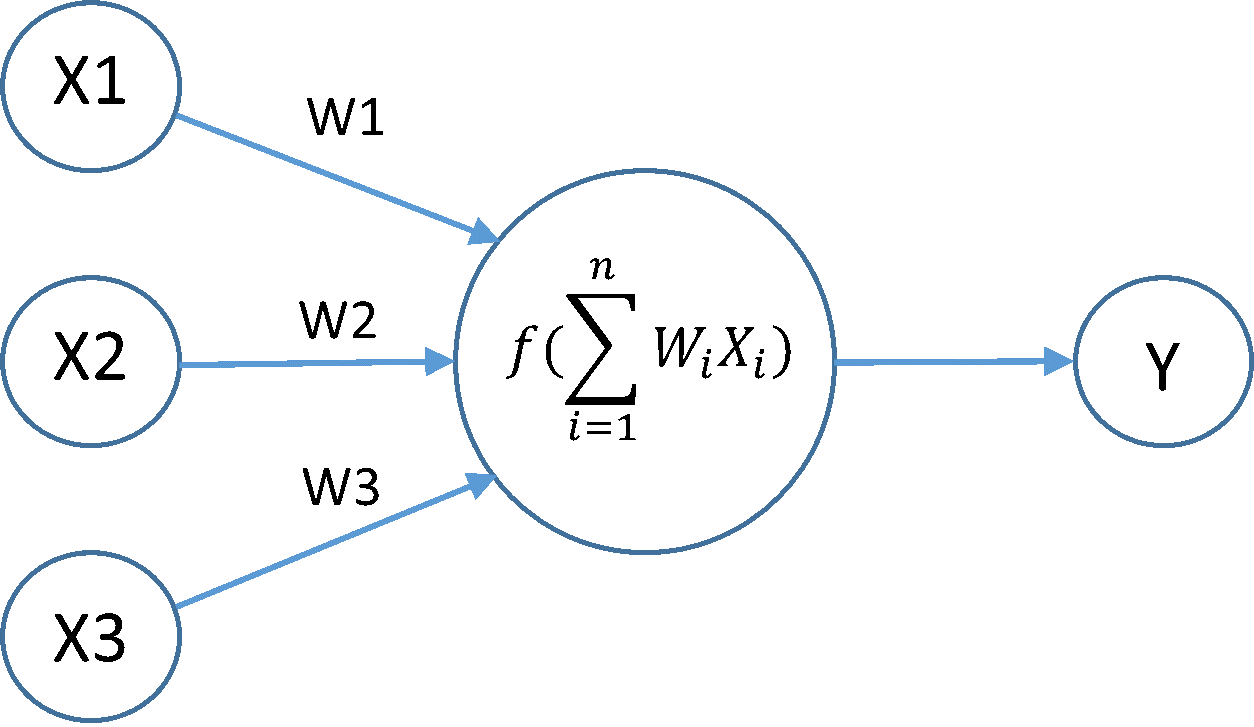
\includegraphics[scale=1]{ANN_diagram}};
			\node [num, anchor=west] at(ANN.north east)  {NUMBER 1};
			\node [num, anchor=west] at(ANN.east) {Layers};
			\node [num, anchor=west] at(ANN.south east) {NUMBER 3};
			\end{scope}
			\end{tikzpicture}
		}
	\end{columns}

	
	\block{AI}{
	}
	\column{.5}
	\block{Wetware}{
	}
	\block{Pervasive Computing}{
		\begin{center}
			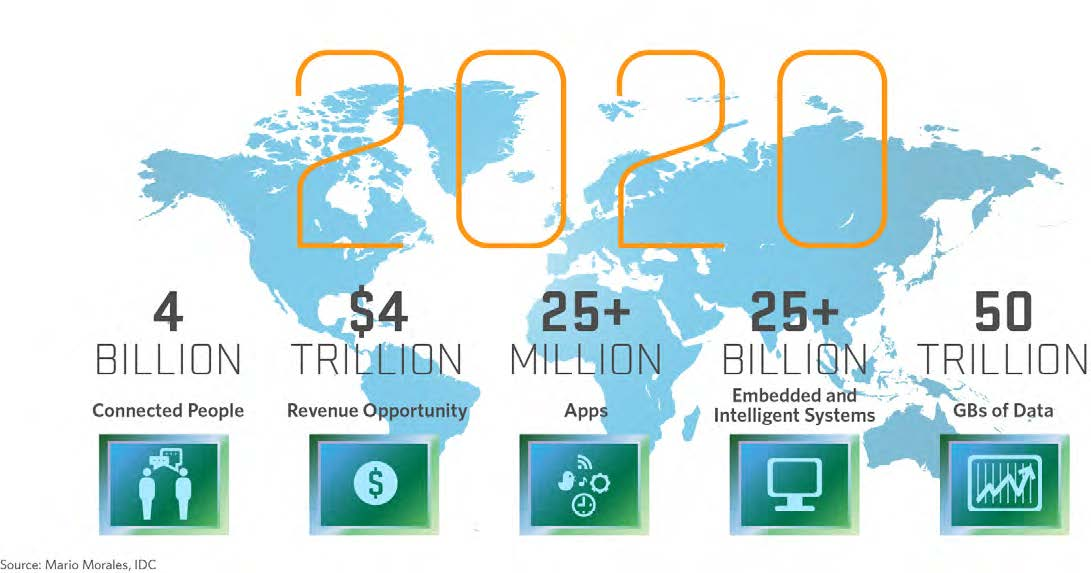
\includegraphics[width=.8\textwidth]{PervComp_IoT}
		\end{center}
	}
\end{document}